% !TeX encoding = UTF-8
% !TeX spellcheck = de_DE

\documentclass[biblatex]{lni}
\addbibresource{lni-paper-example-de.bib}


\usepackage{booktabs} % Schöne Tabellen mittels \toprule, \midrule, \bottomrule
\usepackage[]{blindtext} % Zu Demonstrationszwecken
\usepackage{fancyhdr}
\usepackage{acronym}

%% Sietenzahlen
\pagestyle{fancy}
\fancyhf{}
\fancyfoot[C]{\thepage}
\renewcommand{\headrulewidth}{0pt}

\begin{document}

\begin{titlepage}
  \centering
  \vspace*{0.5cm}

  {\scshape\LARGE Fallstudie \par}

  {\huge\bfseries
    Analyse von Web Applikations-Technologien:
  \par
  }
  {\Large\itshape Am Beispiel der Planung einer GLS Quiz App\par}

  \vspace{1cm}

  {\Large\textbf{Eingereicht von: }}\\
  Nicolas Fritz \\
  E-Mail: nicolasnoah.fritz@gls-germany.com

  \vspace{1cm}

  {\Large\textbf{Eingereicht bei: }}\\
  Hochschule Fulda \\
  Leipziger Straße 123 \\
  36037 Fulda \\
  Lehrperson: Prof. Dr. Brigit Bomsdorf

  \vspace{1cm}

  {\Large\textbf{Unternehmen: }}\\
  GLS Germany GmbH & Co. OHG \\
  Betreuung: Laura Alles, Patrick Weppler

  \vfill

  {\large \today\par}
\end{titlepage}

\tableofcontents
\listoffigures
\newpage

\section*{Abkürzungsverzeichnis}
\begin{acronym}[Bash]
  \acro{WebApp}{Webanwendung}
  \acro{GUI}{Graphical User Interface, also Benutzeroberfläche}
  \acro{HTML}{Hypertext Markup Language}
  \acro{CSS}{Cascading Style Sheets}
  \acro{JS}{JavaScript}
\end{acronym}
\newpage

\section{Einleitung}
Diese Fallstudie mit dem Titel „Analyse von Web Applikations-Technologien: Am Beispiel der Planung einer GLS Quiz App“
wurde im Fachbereich Angewandte Informatik von Nicolas Fritz im Unternehmen GLS Germany GmbH & Co. OHG erstellt.
Die Betreuung im Unternehmen erfolgte durch Patrick Weppler für den technischen Teil und Laura Alles für den konzeptionellen Teil.
An der Hochschule wurde die Arbeit von Prof. Dr. Birgit Bomsdorf betreut.
Das Thema wird anhand des Fallbeispiels einer GLS Quiz App erläutert und analysiert.

\subsection{Hintergrund und Motivation}
Software wird zunehmend komplexer und enthält immer mehr Funktionen, von denen viele standardisiert und wiederkehrend sind.
Je größer das Projekt, desto schwieriger wird es, den Überblick zu behalten – insbesondere bei Webanwendungen,
die sich kontinuierlich weiterentwickeln und fortlaufend programmiert werden.
Um den Überblick zu bewahren, sind daher Konzepte notwendig, die eine Erweiterbarkeit sicherstellen.
Außerdem muss Software skalierbar und gleichzeitig effizient sein.

\\

Ein Beispiel für eine solche Webanwendung, folgend nur WebApp, ist die GLS-Quiz App.
Diese App dient dazu, neue duale Studenten, Auszubildende oder Mitarbeiter mit dem Unternehmen vertraut zu machen.
Sie basiert auf einer zuvor genutzten analogen Version, in der die Nutzer in die Rolle eines Paketboten schlüpfen,
Pakete ausliefern und dabei auf verschiedene Probleme stoßen, die sie durch das Beantworten von Fragen lösen müssen.

\\

Im Verlauf der Konzeptionierung und Umsetzung der App stellte sich heraus,
dass die ursprüngliche analoge Version aufgrund der gewählten Technologie stark vereinfacht werden musste
und die Weiterentwicklung nun deutlich erschwert ist.

\\

Daher benötigen wir eine Lösung,
die eine vorgegebene Struktur bietet und grundlegende Funktionen bereits integriert.
Gleichzeitig müssen einfache Erweiterungsmöglichkeiten gewährleistet sein.

\subsection{Ziel der Fallstudie}

\subsection{Methodik und Vorgehensweise}

\section{Technologieüberblick}
Um die Entwicklung einer WebApp wie der GLS Quiz App besser zu verstehen,
ist es wichtig, die zugrunde liegenden Technologien zu kennen.

\\

Im folgenden Abschnitt werden die Grundlagen geschaffen,
moderne Technologien aufgezeigt und verglichen.
Zusätzlich wird die Zusammenarbeit der wichtigsten Komponenten einer WebApp aufgezeigt.

\subsection{Überblick über moderne Webtechnologien}

Um eine WebApp oder Website zu verstehen oder entwickeln zu können, ist es wichtig, die zugrunde liegende Struktur zu kennen.
Eine wesentliche Unterscheidung ist dabei die zwischen Frontend und Backend.

Das Frontend bezeichnet hierbei den sichtbaren Teil einer WebApp, den der Nutzer direkt erleben kann. \cite{CMSRev}
Anders gesagt ist es das \ac{GUI} einer Anwendung.
Es umfasst alles, was auf dem Bildschirm angezeigt wird, einschließlich Gestaltung und Interaktion.
Das Frontend besteht aus den drei grundlegenden Technologien \ac{HTML}, \ac{CSS} und \ac{JS}.

Die Seite Time4Innovation \cite{T4I} beschreibt die drei Technologien wie folgt: \\
\textbf{\ac{HTML}} ist der grundlegende Aufbau einer Seite.
Es definiert die Struktur und den Inhalt. \\
\textbf{\ac{CSS}} ist für das Design zuständig.
Die mit \ac{HTML} definierten Elemente werden hiermit gestaltet, also zum Beispiel Farben, Schriftarten und Abstände. \\
\textbf{\ac{JS}} ist für die Interaktion zuständig.
Alles was nicht mittels \ac{HTML} und \ac{CSS} umgesetzt werden kann, wird mit \ac{JS} realisiert.

Ein Frontend für eine WebApp besteht typischerweise aus diesen 3 Technologien oder Abwandlungen dieser. \cite{CoU}
Der Grund dafür ist, dass der Browser nur diese Sprachen versteht und sie für die Benutzer interpretiert.
Das ist der Grund dafür, dass diese Sprachen auch als \texttt{clientseitige} Sprachen bezeichnet werden.

\\

Das Backend hingegen benutzt \texttt{serverseitige} Sprachen. \cite{CMSRev}
Es ist verantwortlich für die Verwaltung von Daten und Verarbeitung von Benutzerinteraktionen.
Dabei umfasst es den Server, der Anfragen vom Frontend entgegennimmt und verarbeitet,
sowie die Datenbank, die unter anderem zur Speicherung der Daten dient.

Die Sprachen variieren stark und sind abhängig von den Anforderungen der Anwendung.
Typische serverseitige Sprachen sind \textbf{Java}, \textbf{Python} oder \textbf{PHP}.
Eine Besonderheit besteht darin, dass auch \ac{JS} serverseitig verwendet werden kann.

\\

Doch wie bereits erwähnt reicht eine Sprache nicht aus, um eine WebApp zu entwickeln.
Heutige WebApps sind komplexer und benötigen daher sogenannte Frameworks.
Eine Definition der Rock the Prototype Seite lautet: \\
\begin{minipage}{\textwidth}
  \textit{
    \\
    \\
    \textbf{"} \\
    Frameworks bieten vorgefertigten Code,
    der als Ausgangspunkt für die Entwicklung von Anwendungen verwendet werden kann. Dies spart Zeit und Mühe,
    da die Entwickler nicht von Grund auf mit der Programmierung beginnen müssen.
    Stattdessen können sie den vorgefertigten Code als Grundlage verwenden und ihn mit eigenem Code ergänzen.
    \\
    \textbf{"} \\
    \Cite{RtP}
    \\
  }
\end{minipage}

Also bedeutet das,
dass Frameworks den Entwicklungsprozess durch die Bereitstellung von Standardlösungen und wiederverwendbarem Code beschleunigen.
Entwickler können auf diese vorgefertigten Komponenten zurückgreifen,
um wiederkehrende Aufgaben zu automatisieren und sich auf die individuellen Anforderungen ihrer WebApp zu konzentrieren.
Frameworks helfen dabei, die Komplexität zu bewältigen,
indem sie eine strukturierte Basis bieten, auf der Entwickler ihre spezifischen Funktionen aufbauen können.

Im folgenden Abschnitt werden wir 3 Frontend- und Backend-Frameworks etwas genauer betrachten und miteinander vergleichen.

\subsection{Frontend-Technologien im Vergleich: VueJS, Angular und React}


\Cref{fig:fetrends} zeigt den Verlauf der Fragen zu Webtechnologien auf Stack Overflow,
einer sehr bekannten Plattform für Programmierfragen, über die relevanten Jahre.

\begin{figure}
  \centering
  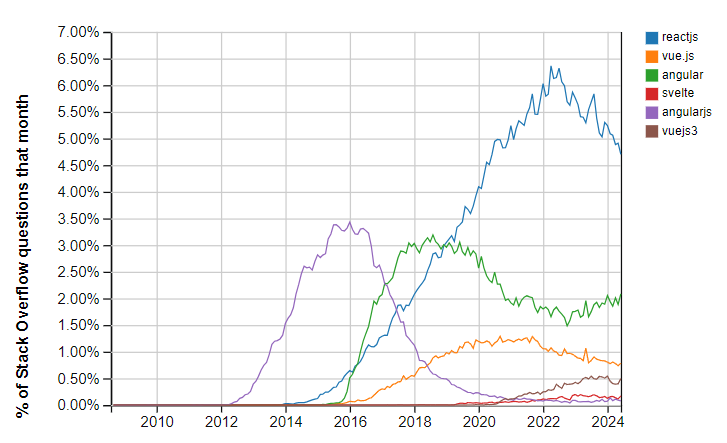
\includegraphics[width=.8\textwidth]{fetrends}
  \caption{Stackoverflow Fragen Frontend-Frameworks.}
  \label{fig:fetrends}
  \vspace{-0.3cm}
  \begin{center}
    \footnotesize Quelle: \cite{SOTrend}
  \end{center}
\end{figure}

Die Grafik bietet zwar keinen umfassenden Einblick in die Nutzung von Frameworks in Unternehmen,
liefert jedoch eine grobe Orientierung darüber, welche Technologien Entwickler auch privat verwenden und somit bevorzugen.


- nur die Fragen auf Stackoverflow, nicht so guten Einblick in Firmen Nutzung, aber schafft trotzdem eine grobe Richtung, was die Entwickler auch privat benutzen würden
- Angular mit angularjs eine der ersten Frontend-Frameworks die aufkamen
- Mit der neuen Version Angular 2 wurde das Framework komplett neu geschrieben und angularjs wurde langsam abgelöst
- fiel jedoch in der Beliebtheit und wurde von React 2019 überholt
- vue erkennt man das selbe wie angularjs und angular mit vue.js und vue3
- vue ist unter angular
- react hat sehr an beliebtheit gewonnen

\subsection{Backend-Technologien im Vergleich: Express, Springboot und Django}
\subsection{Wie arbeiten Backend und Frontend zusammen?}

\section{Die GLS Quiz App}
\subsection{Ist-Zustand der App}
\subsection{Ursprüngliches Konzept}
\subsection{Probleme bei der Umsetzbarkeit des ursprünglichen Konzepts}
\subsection{Konzeptentwicklung zur Bewältigung der Herausforderungen}

\section{Test-Implementierung}
\subsection{Das Demo Projekt}
\subsection{Umsetzung}
\subsection{Ergebnisse und erlangtes Wissen}

\section{Schlussfolgerung und Ausblick}

\newpage
\printbibliography

\end{document}
